\documentclass[problem]{mcs}

\begin{pcomments}
  \pcomment{FP_and_circuit_shorter}
  \pcomment{shorter version of FP_and_circuit from s17.cp2w, f15.midterm1}
  \pcomment{revised by ARM to use depth parameter instead of \# inputs.}
  \pcomment{s17.mid1}
\end{pcomments}

\pkeywords{
  circuit
  digital
  and
  tree
}

\newcommand{\dpn}[1]{\text{gate}\#(#1)}

%%%%%%%%%%%%%%%%%%%%%%%%%%%%%%%%%%%%%%%%%%%%%%%%%%%%%%%%%%%%%%%%%%%%%
% Problem starts here
%%%%%%%%%%%%%%%%%%%%%%%%%%%%%%%%%%%%%%%%%%%%%%%%%%%%%%%%%%%%%%%%%%%%%

\begin{problem}
A $k$-bit $\QAND$-circuit is a digital circuit that has $k$ 0-1 valued
inputs\footnote{Following the usual conventions for digital circuits,
  we're using 1 for the truth value \true\ and 0 for \false.}
$d_0,d_1,\dots,d_{k-1}$ and one 0-1-valued output variable whose value
will be
\[
d_0 \QAND d_1 \QAND \cdots \QAND d_{k-1}.
\]
$\QOR$-circuits are defined in the same way, with ``\QOR'' replacing
``\QAND.''

\bparts

\ppart\label{ANDSandORS} Suppose we want an \QOR-circuit but only have
a supply of \QAND-circuits and some \QNOT-gates (``inverters'') that
have one 0-1 valued input and one 0-1 valued output.  We can turn an
\QAND-circuit into an \QOR-circuit by attaching a \QNOT-gate to each
input of the \QAND-circuit and also attaching a \QNOT-gate to the
output of the \QAND-circuit.  This is illustrated in
Figure~\ref{fig:demorg-circuit}.
\begin{figure}
  \includegraphics[height=1.25in]{}%OR-from-AND}
\caption{\TBA{OR-from-AND figure}}
%  \caption{A \QOR-circuit from a \QAND-circuit.}
  \label{fig:demorg-circuit}
\end{figure}
Briefly explain why this works.

\examspace[1in]

\begin{solution}
Negating the inputs and the output of a $k$-bit \QAND-circuit with
inputs $d_0,d_1,\dots,d_{k-1}$ turns it into a circuit that whose
output value will be
\[
\QNOT(\bar{d_0} \QAND \bar{d_1} \QAND \cdots \QAND \bar{d_{k-1}}),
\]
which by DeMorgan's Law is equivalent to
\[
d_0 \QOR d_1 \QOR \cdots \QOR d_{k-1}.
\]
\end{solution}
\eparts

\medskip

Large digital circuits are built by connecting together smaller
digital circuits as components.  One of the most basic components is a
two-input/one-output \QAND-gate that produces an output value equal to
the \QAND\ of its two input values.  So according the definition in
part~\eqref{ANDSandORS}, a single \QAND-\emph{gate} is a 1-bit
\QAND-\emph{circuit}.

We can build up larger \QAND-circuits out of a collection of
\QAND-gates in several ways.  For example, one way to build a 4-bit
\QAND-circuit is to connect three \QAND-gates as illustrated in
Figure~\ref{fig:AND-tree-4}.
\begin{figure}
  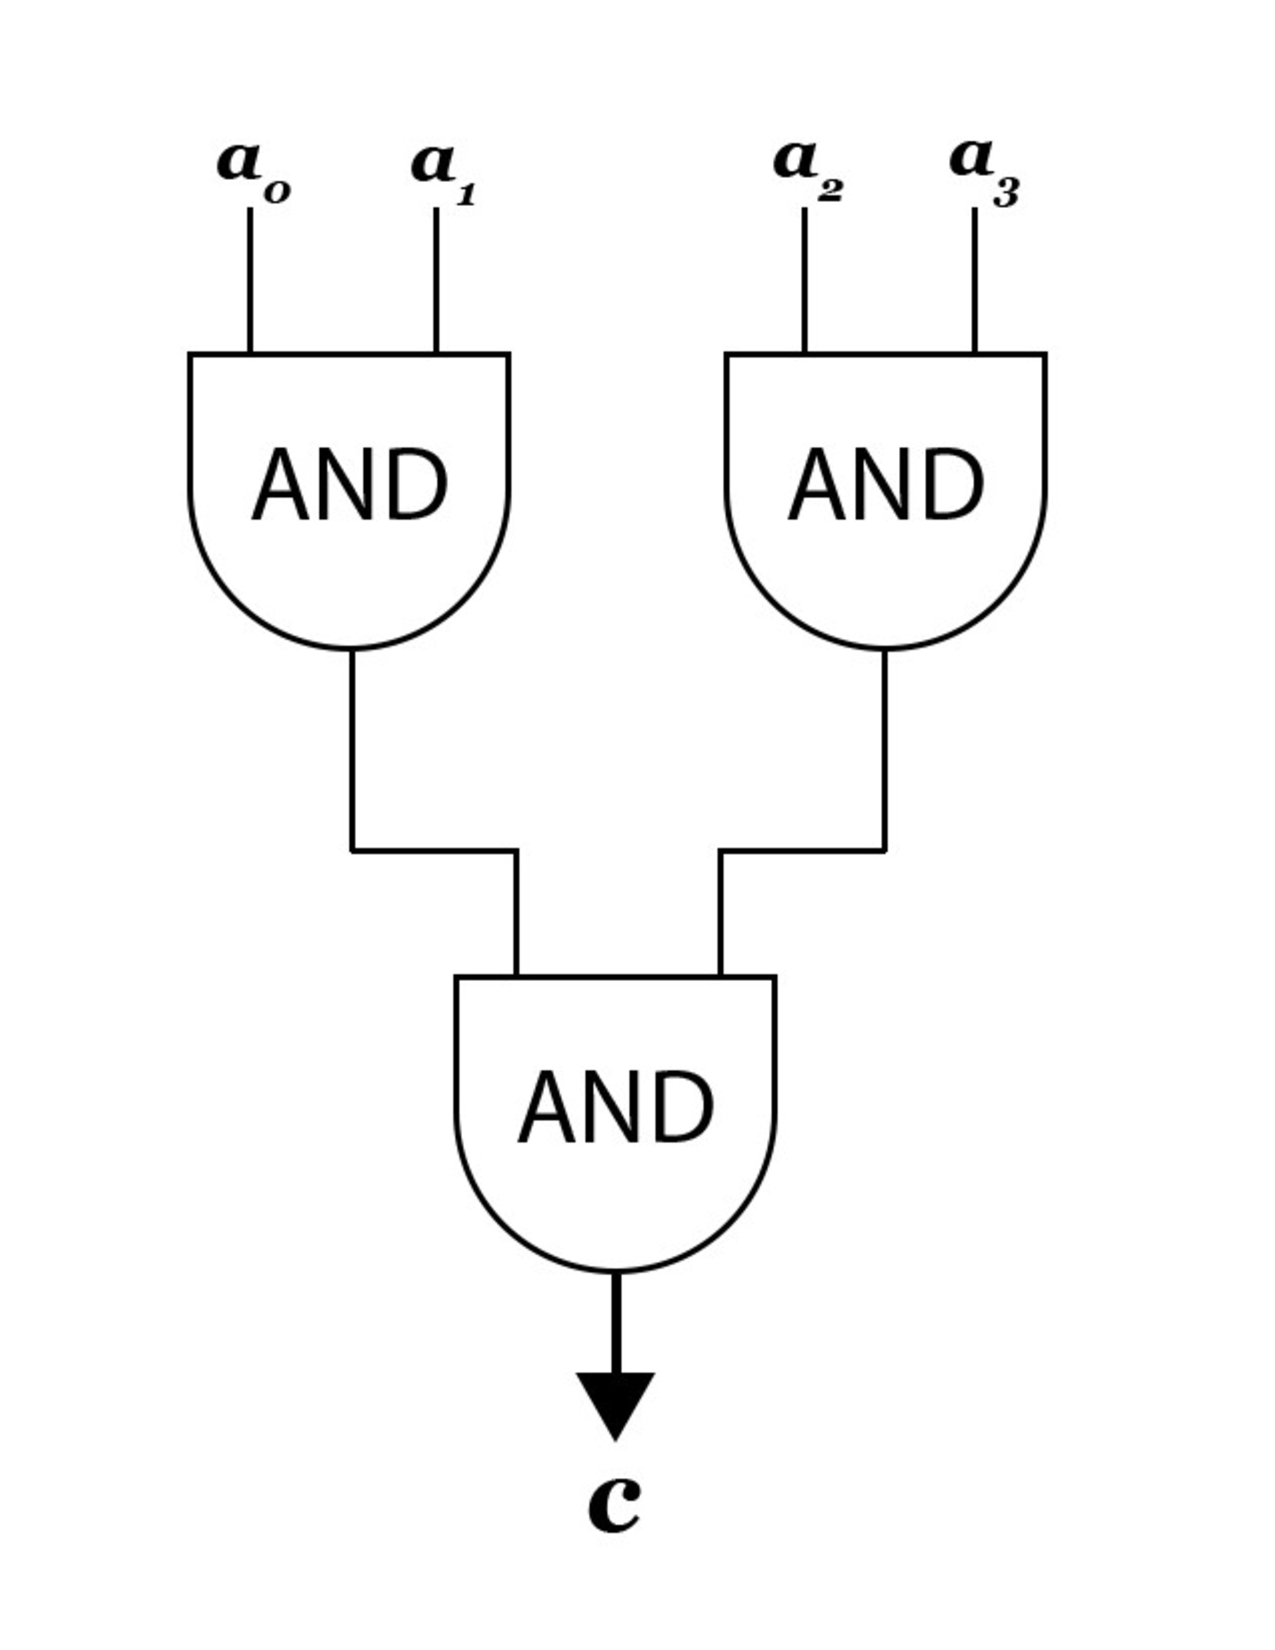
\includegraphics[height=1.25in]{AND_tree_4}
  \caption{A $4$-bit \QAND-circuit.}
  \label{fig:AND-tree-4}
\end{figure}

More generally, a \emph{depth-$n$ tree-design
  \QAND-circuit}---``depth-$n$ circuit'' for short---has $2^n$ inputs
and is built from two depth-$(n-1)$ circuits by using the outputs of
the two depth-$(n-1)$ circuits as inputs to a single \QAND-gate.  This
is illustrated in Figure~\ref{fig:AND-tree-n}.
\begin{figure}
  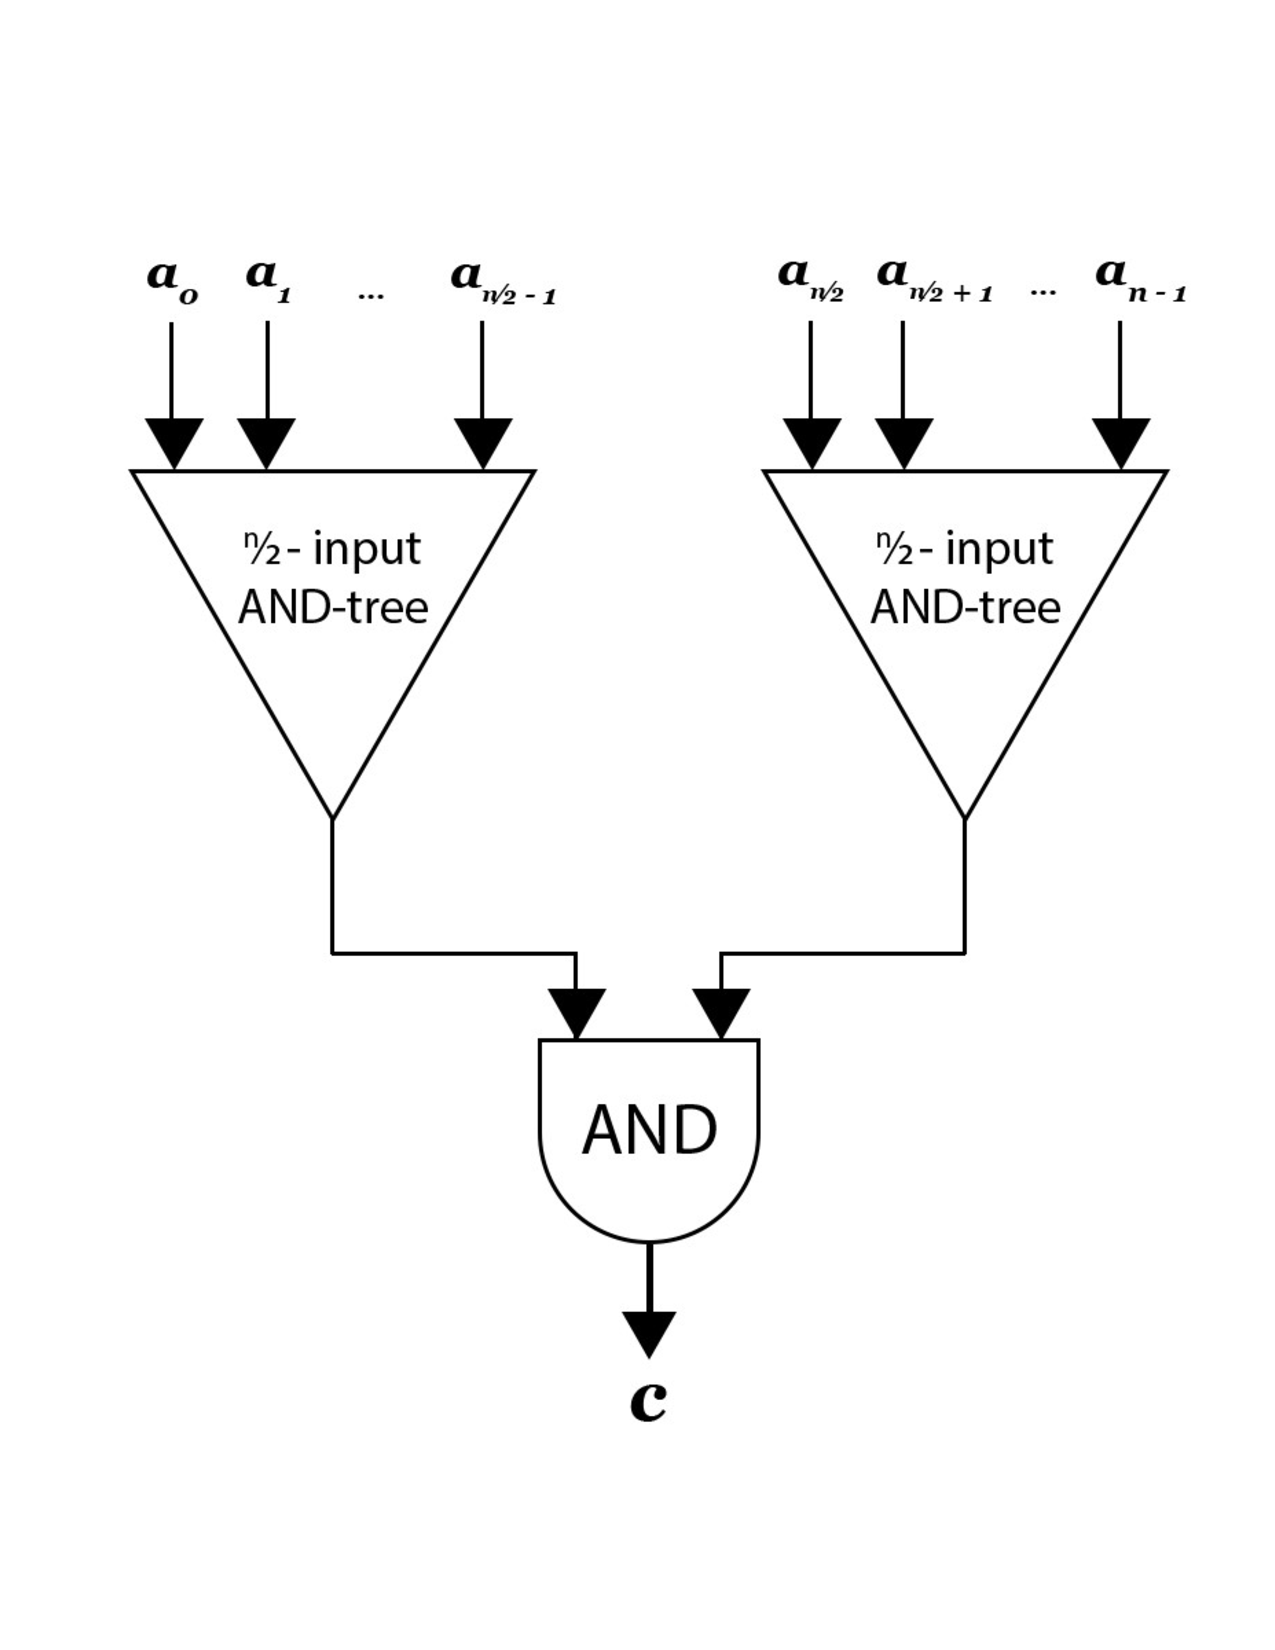
\includegraphics[height=2.5in]{AND_tree_recursive}
  \caption{An $n$-bit tree-design $\QAND$-circuit.}
  \label{fig:AND-tree-n}
\end{figure}
So the 4-bit \QAND-circuit in Figure~\ref{fig:AND-tree-4} is a depth-2
circuit.  A depth-1 circuit is defined simply to be a single
\QAND-gate.

\iffalse
A depth-0 $\QAND$-circuit is just a wire connecting the single input
to the output, so it has no \QAND-gates.
\fi

\bparts

\ppart Let $\dpn{n}$ be the number of \QAND-gates in a depth-$n$
circuit.  Use the Well Ordering Principle to prove that
\[
\dpn{n} = 2^n-1
\]
for all $n \geq 1$.

\examspace[5in]

\begin{solution}
\begin{proof}
From the definition of depth-$n$ circuit, we have
\begin{equation}\tag{*}
\dpn{n+1} = 2\dpn{n} + 1.
\end{equation}
for $n \geq 1$.

Suppose for the sake of contradiction that $\dpn{n}$ is not equal to
$2^n-1$ for some $n \geq 1$.  Then by the Well Ordering Principle,
there is a minimum number $m \geq 1$ with $\dpn{m} \neq 2^m-1$.

Now a depth-1 circuit has $1 = 2^1-1$ gates, so $m$ must be greater
than 1.  Since $m$ is the minimum number with $\dpn{m}\neq 2^m-1$ and
$m-1 \geq 1$, we have $\dpn{m-1} = 2^{m-1}-1$.  Now by~(*), we have
\[
\dpn{m} = 2\dpn{m-1} + 1 = 2(2^{m-1}-1) + 1 = 2^m -2 + 1 = 2^m -1,
\]
contradicting the assumption that $\dpn{m}$ has a different value.

This contradiction implies that $\dpn{n}$ must equal $2^n-1$ for all
$n \geq 1$.
\end{proof}
\end{solution}

\eparts

\end{problem}

%%%%%%%%%%%%%%%%%%%%%%%%%%%%%%%%%%%%%%%%%%%%%%%%%%%%%%%%%%%%%%%%%%%%%
% Problem ends here
%%%%%%%%%%%%%%%%%%%%%%%%%%%%%%%%%%%%%%%%%%%%%%%%%%%%%%%%%%%%%%%%%%%%%

\endinput

\iffalse
Serial is described by
the formulas:
\begin{align*}
  c_1     & \eqdef a_1 \QAND\ a_0\\
  c_2     & \eqdef a_2 \QAND\ c_1\\
  c_3     & \eqdef a_3 \QAND\ c_2\\
  & \vdots\\
  c_{n-1}  & \eqdef a_{n-1} \QAND\ c_{n-2}\\
  c       & \eqdef c_{n-1}.
\end{align*}


The tree design is
described by formulas involving binary variables $t_y$ where
$y$ ranges over binary strings of length $\leq k$.  Any such
positive length string $y$ is a binary representation of a
nonnegative integer $\binnum{y}$ less than $n$.  For example,
\[
\binnumt{00001} = 1, \quad \binnumt{010} = 2, \quad \binnumt{11} =
3, \binnumt{110} = 6, \quad \binnumt{0111} = 7.
\]

We begin by defining
\[
t_y \eqdef a_{\binnum{y}} \text{   (for $y$ of length $k$)}.
\]
For $y$ of length less than $k$, define
\[
t_{y} \eqdef t_{y\mtt{0}} \QAND\ t_{y\mtt{1}}
\]
So
\begin{align*}
  t_{\lambda} & \eqdef t_{\mtt{0}} \QAND\ t_{\mtt{1}}\\
  t_{0} & \eqdef t_{\mtt{00}} \QAND\ t_{\mtt{01}}\\
  t_{1} & \eqdef t_{\mtt{10}} \QAND\ t_{\mtt{11}}\\
  t_{00} & \eqdef t_{\mtt{000}} \QAND\ t_{\mtt{001}}\\
  & \vdots
\end{align*}
Finally, the output $c$ is
\[
c  \eqdef t_{\lambda}.
\]
\fi
